%%%%%%%%%%%%%%%%%%%%%%%%%%%%%%%%%%%%%%%%%%%%%%%%%%%%%%%%%%%%
%%  This Beamer template was created by Cameron Bracken.
%%  Anyone can freely use or modify it for any purpose
%%  without attribution.
%%
%%  Last Modified: January 9, 2009
%%

\documentclass[xcolor=x11names,compress]{beamer}
\setbeamertemplate{navigation symbols}{}
\setbeamertemplate{footline}[page number]

%% General document %%%%%%%%%%%%%%%%%%%%%%%%%%%%%%%%%%
\usepackage{graphicx}
\usepackage{tikz}
\usetikzlibrary{decorations.fractals}
%%%%%%%%%%%%%%%%%%%%%%%%%%%%%%%%%%%%%%%%%%%%%%%%%%%%%%


%% Beamer Layout %%%%%%%%%%%%%%%%%%%%%%%%%%%%%%%%%%
\useoutertheme[subsection=false,shadow]{miniframes}
\useinnertheme{default}
\usefonttheme{serif}
\usepackage{palatino}

\setbeamerfont{title like}{shape=\scshape}
\setbeamerfont{frametitle}{shape=\scshape}

\setbeamercolor*{lower separation line head}{bg=DeepSkyBlue4} 
\setbeamercolor*{normal text}{fg=black,bg=white} 
\setbeamercolor*{alerted text}{fg=red} 
\setbeamercolor*{example text}{fg=black} 
\setbeamercolor*{structure}{fg=black} 
 
\setbeamercolor*{palette tertiary}{fg=black,bg=black!10} 
\setbeamercolor*{palette quaternary}{fg=black,bg=black!10} 

\renewcommand{\(}{\begin{columns}}
\renewcommand{\)}{\end{columns}}
\newcommand{\<}[1]{\begin{column}{#1}}
\renewcommand{\>}{\end{column}}
%%%%%%%%%%%%%%%%%%%%%%%%%%%%%%%%%%%%%%%%%%%%%%%%%%


%% Titlepage without header %%%%%%%%%%%%%%%%%%%%%%
\makeatletter
    \newenvironment{withoutheadline}{
        \setbeamertemplate{headline}[default]
        \def\beamer@entrycode{\vspace*{-\headheight}}
    }{}
\makeatother
%%%%%%%%%%%%%%%%%%%%%%%%%%%%%%%%%%%%%%%%%%%%%%%%%%


%% Graphics path %%%%%%%%%%%%%%%%%%%%%%%%%%%%%%%%%
\graphicspath{{.}{images/}}
\DeclareGraphicsExtensions{.pdf, .png, .jpg}
%%%%%%%%%%%%%%%%%%%%%%%%%%%%%%%%%%%%%%%%%%%%%%%%%%


%% aliases %%%%%%%%%%%%%%%%%%%%%%%%%%%%%%%%%%%%%%%
\usepackage{amsmath}	% need for math
\usepackage{graphicx}   % need for figures
\usepackage{bbm}		% need for bold indicators 1(i<j)
\usepackage{framed}		% need for framed environment
\usepackage{color}		% need for colorful fonts

\usepackage{fancybox}	% for fancy boxes

\usepackage{amssymb}
\usepackage{amsmath}
\usepackage{amsthm}
%\usepackage{bbm} % for hollow 1
\usepackage{dsfont} % for hollow 1 with Type 1 fonts
\newcommand{\Sn}{\mathbb{S}_n}
\newcommand{\fixme}[1]{{\bf [FIXME: #1]}}
%\newtheorem{thm}{Theorem}
\newcommand{\RR}{\mathbb{R}}    %reals
\newcommand {\br}[1]{\left(#1\right)}
\newcommand {\sqb}[1]{\left[#1\right]}
\newcommand {\cbr}[1]{\left\{#1 \right\}}
\newcommand{\xb}{\mathbf{x}}
\newcommand{\ub}{\mathbf{u}}
\newcommand{\wb}{\mathbf{w}}
\newcommand {\nm}[1]{\Arrowvert\, #1 \,\Arrowvert}
\newcommand {\abs}[1]{\left\vert\, #1 \,\right\vert}
\newcommand{\EE}{\mathbb{E}}
\newcommand{\wh}{\widehat{\wb}}
\newcommand{\Rh}{\widehat{R}}
\newcommand {\OMIT}[1]{}               % to ignore things

\newcommand{\sgn}{\operatorname{sgn}}
%%%%%%%%%%%%%%%%%%%%%%%%%%%%%%%%%%%%%%%%%%%%%%%%%%


\begin{document}

\begin{withoutheadline}
	\begin{frame}
		\begin{tikzpicture}[align=center]
			\coordinate (o) at (current page.center);
			\coordinate[xshift=-64.3mm, yshift=-118.5mm] (vt0) at (o);
      \coordinate[xshift=-64.3mm, yshift=-136.5mm] (vt1) at (o);
      \draw[darkgray] (vt0) -- (vt1);
			\node[xshift=-75mm, yshift=-126.5mm] at (o) {
        
\includegraphics[height=1.8cm]{preamble/Logo_MINES_ParisTech}
      };
      \node[xshift=-50mm, yshift=-126.5mm] at (o) {
        
\includegraphics[height=1.2cm]{preamble/logo-psl}
      };
		\end{tikzpicture}
		
		\title{Rank-based Molecular Prognosis and Network-guided Biomarker Discovery for Breast Cancer}
		\author{
			Yunlong Jiao\\
			{\scriptsize Supervised by Jean-Philippe Vert}
		}
		\institute{{\it Mines ParisTech}}
		\date{PhD Defense, September 11, 2017}
		\titlepage
	\end{frame}
\end{withoutheadline}


\section{\scshape Introduction}

\begin{frame}{Cancer prognosis}
	
	\begin{itemize}
		\item Prognosis is an estimate of the likely course or outcome
of cancer patients.
	\end{itemize}
	
	\(
	\<{0.4\linewidth}
	\fbox{
		\parbox{0.8\columnwidth}{
		Clinical information
		}
	}
	\begin{equation*}
		\left\{
		\begin{array}{l}
			\textrm{Age at diagnosis} \\
			\textrm{Tumor size} \\
			\textrm{Cancer type/stage} \\
			\textrm{Positive lymph nodes} \\
			\cdots
		\end{array}
		\right.
	\end{equation*}
	
	\only<2->{
	\fbox{
		\parbox{0.95\columnwidth}{
		\& Genomic information
		}
	}
	\begin{equation*}
		\left\{
		\begin{array}{l}
			\textrm{{\only<3>{\color{red}}Gene expression}} \\
			\textrm{Copy number variation} \\
			\cdots
		\end{array}
		\right.
	\end{equation*}
	}
	\>
	
	\<{0.2\linewidth}
	\begin{figure}
	\begin{center}
		\only<1>{
		
\includegraphics[width=0.8\columnwidth]{slides/doctor}
		}
		\only<2->{
		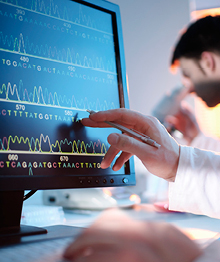
\includegraphics[width=1.2\columnwidth]{slides/Bioinfo}
		}
	\end{center}
	\end{figure}
	\>
	
	\<{0.4\linewidth}
	\fbox{
		\parbox{0.9\columnwidth}{
		\only<1>{High/low risk of 5-year relapse}
		\only<2->{
			{\only<3>{\color{red}}Survival classification or survival analysis}
		}
		}
	}
	\>
	\)
	
\end{frame}


\begin{frame}{Supervised analysis of gene expression data}
	
	\begin{itemize}
		\item Data: 
		\begin{itemize}
			\item[-] $X$ denotes $p$-gene expression profiles of $n$ cancer patients.
			\item[-] $\mathbf{y}$ denotes the prognosis class or survival time of the $n$ patients.
		\end{itemize}
		
		\item Goal: Learn to predict $y$ from a patient's profile $\mathbf{x}$.
		\begin{figure}
		\begin{center}
			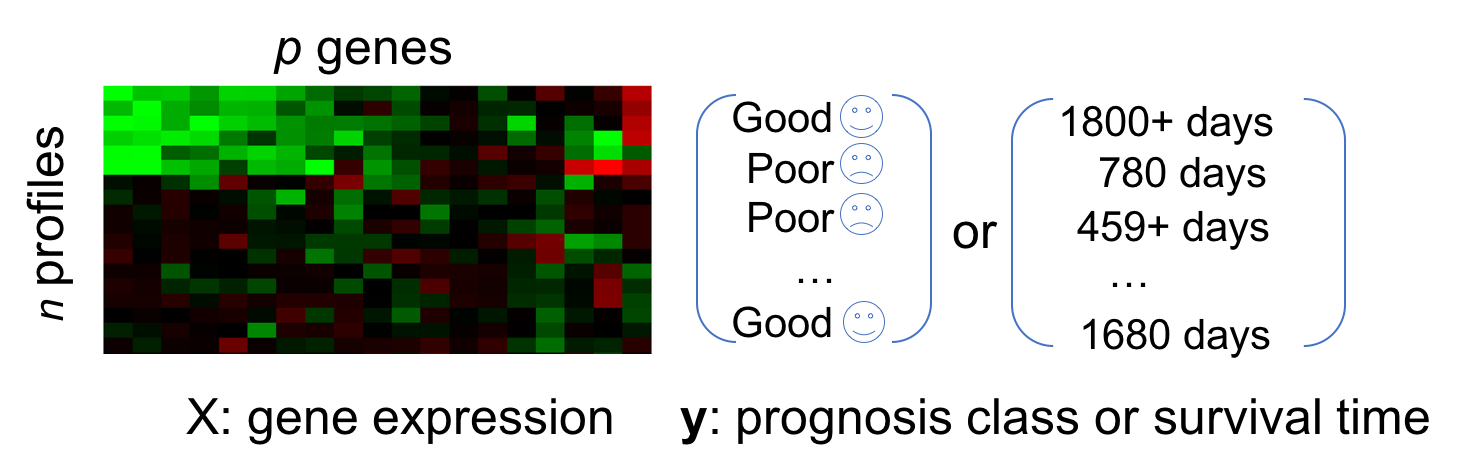
\includegraphics[width=0.8\linewidth]{slides/prognosis}
			\vskip -0.1in
			\caption{{\scriptsize Prognosis classification (good vs. poor) or survival analysis of gene expression data.}}
		\end{center}
		\end{figure}
		
		\item<2-> Challenge:
		\begin{itemize}
			\item[-] High-dimensional ($n \ll p$) and high-throughput measurements (Project 1).
			\item[-] Interpretability of gene selection (Project 2).
		\end{itemize}
	\end{itemize}
\end{frame}







\begin{frame}[allowframebreaks]{References}
	
	\footnotesize
	\bibliography{mybib}
	\bibliographystyle{apalike}
	
\end{frame}



\end{document}
